\begin{figure}[h]
	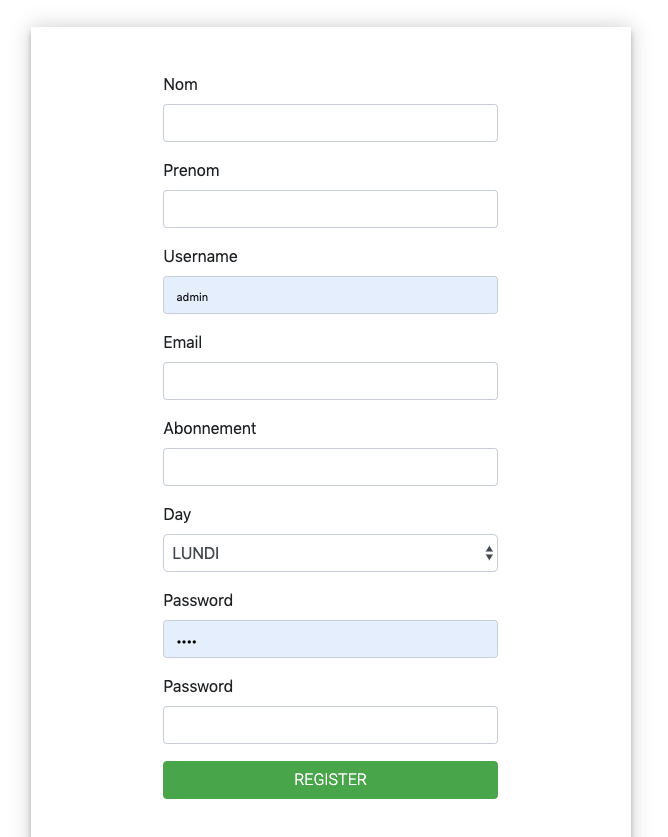
\includegraphics[width=0.5\textwidth,center]{Figures/us1-1}
	\caption{Formulaire d'inscription}
\end{figure}

\vspace{\baselineskip}
\begin{enumerate}
	\item L'utilisateur rentre s'est information dans le formulaire. 
	\item L'utilisateur sélectionne le type de session au quelle il est inscrit. 
	\item L'utilisateur clique sur \textit{Register} et attend la redirection. 
\end{enumerate}

\newpage
\subsubsection{Gestion des erreurs et sécurité}
	\paragraph{}
		\begin{itemize}
			\item L'utilisateur dois remplir tout les champs, si un champs est manquant une erreur apparaitra. 
			\item Le nom d'utilisateur et l'adresse Email son unique dans le système, si il entre un Email ou nom d'utilisateur deja existant une erreur lui dira de changer la faute.
			\item L'utilisateur dois confirmer sont mot de passe, si les mots de passe sont différent ou plus petit que 6 charactère il y aura une erreur.
		\end{itemize}
		
\subsubsection{Diagramme de séquence}
	\begin{figure}[h]
		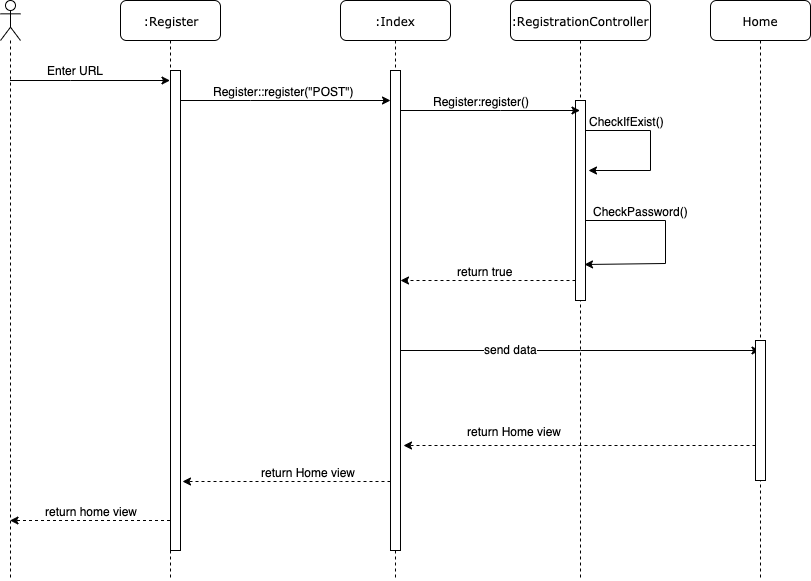
\includegraphics[width=0.8\textwidth,center]{Diagramme/sequence-us1}
		\caption{Diagramme de séquence de l'enregistrement d'un nouvelle utilisateur. }
	\end{figure}
	
	
\subsubsection{Script concernés}
	\begin{itemize}
		\item \Href{https://github.com/victorsmits/Aquabike/blob/master/backend/src/Controller/RegistrationController.php}{RegistrationController.php}
		\item \Href{https://github.com/victorsmits/Aquabike/blob/master/backend/templates/registration/register.html.twig}{register.html.twig}
		\item \Href{https://github.com/victorsmits/Aquabike/blob/master/backend/src/Entity/Person.php}{Person.php}
	\end{itemize}